% basic style definitions for lecture notes in presentation mode.
% based on material from J. W. Langelaan, August 16, 2010

% Vitor Valente, August 2024

\documentclass[times,12pt]{beamer}

\setbeamercolor{background canvas}{bg=white} % Background is set to white
\setbeamercolor{normal text}{fg=black}
\setbeamercolor{alerted text}{fg=black}
\setbeamercolor{example text}{fg=black}
\setbeamercolor{structure}{fg=black} % Section headers, etc.

\setbeamerfont{section title}{size=\small}
\setbeamerfont{frametitle}{size=\large}
\setbeamerfont{normal text}{size=\small}

\setbeamertemplate{navigation symbols}{}

\setbeamertemplate{itemize subitem}[circle]

\setbeamerfont{normal text}{size=\footnotesize}
\setbeamerfont{itemize item}{size=\footnotesize}
\setbeamerfont{itemize text}{size=\footnotesize}

\usepackage{graphicx}
\usepackage{amsmath}  % For mathematical symbols
\usepackage{graphicx} % For including images
\usepackage{hyperref} % For clickable links
\usepackage{subcaption}
\usepackage{tikz} % For block diagrams
\usetikzlibrary{positioning}

\usepackage{ragged2e}
\apptocmd{\frame}{}{\justifying}{} % Allow optional arguments after frame.

\usepackage{xcolor}

% define an environment that prints out notes to self in red if \printnotes is true, in white (on white paper,
% hence invisible) otherwise. Printing notes in white will leave space for student notes...
\newif\ifprintnotes
\newenvironment{mynotes}
{
	\ifprintnotes
		\color{red}
	\else
		\color{white}
	\fi
}
{
	\color{black}
}

% !TEX root = Lecture03.tex
\usepackage{pgfpages}
\usepackage[absolute,overlay]{textpos}

\usetikzlibrary{calc}
\usetikzlibrary{arrows.meta, positioning}

% For printing purposes, 2 slides per page with borders
\pgfpagesuselayout{2 on 1}[letterpaper,border shrink=5mm]
\pgfpageslogicalpageoptions{1}{border code=\pgfusepath{stroke}}
\pgfpageslogicalpageoptions{2}{border code=\pgfusepath{stroke}}
\pgfpageslogicalpageoptions{3}{border code=\pgfusepath{stroke}}
\pgfpageslogicalpageoptions{4}{border code=\pgfusepath{stroke}}

% Title Page Information
\title[AERSP304]{Reference Frames Continued and Examples}
\subtitle{AERSP 304 - Dynamics and Control of \\ Aerospace Systems}
\author[V. T. Valente]{V.T. Valente}
\institute[Penn State University]{Penn State University}
\date{January 16, 2026}

\setlength{\itemsep}{0.0cm}
\setlength{\parsep}{0cm}

\begin{document}
{
%\setbeamertemplate{footline}[text line]{\parbox{\linewidth}{\vspace*{-8pt}Some material in this presentation has been adapted from slides developed by Dr. Joe Horn.}}
\frame{\titlepage}
}
\small

% \begin{center}
%     \begin{tikzpicture}[scale=0.95, line cap=round, line join=round]
%         % origin
%         \coordinate (O) at (0,0);

%         % inertial (N) axes
%         \draw[->, thick] (O) -- (-1.4,-1.2) node[left]  {$\hat{\mathbf n}_1$};
%         \draw[->, thick] (O) -- ( 2.0, 0.0) node[right] {$\hat{\mathbf n}_2$};
%         \draw[->, thick] (O) -- ( 0.0, 2.0) node[above left] {$\hat{\mathbf n}_3$};

%         % body (B) axes
%         \draw[->, thick, blue] (O) -- ( -0.4,-1.4) node[below right] {$\hat{\mathbf b}_1$};
%         \draw[->, thick, blue] (O) -- ( 1.8, 0.8) node[above right] {$\hat{\mathbf b}_2$};
%         \draw[->>, thick, blue] (O) -- ( 0.0, 2.0) node[above right] {$\hat{\mathbf b}_3$};

%         % angle between b2 and n2
%         \draw[->] (0.9,0.0) arc[start angle=0, end angle=23, radius=0.9];
%         \node at (1.1,0.25) {\scriptsize$\theta$};
%     \end{tikzpicture}
% \end{center}

\begin{frame}{Goals for Today}
    \begin{itemize}
        \item Continue review of Frame of References
        \item Analyze velocity and acceleration in different frames
        \item Examples
    \end{itemize}
\end{frame}

\begin{frame}[t]{Reference Frames and Velocity}
    \begin{flushright}
        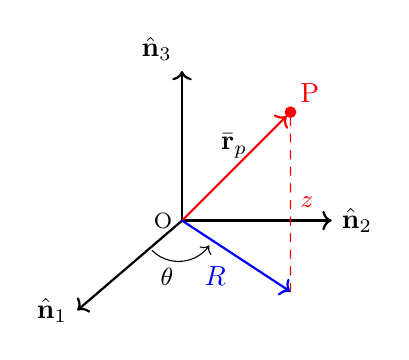
\begin{tikzpicture}[scale=0.95, line cap=round, line join=round]
            % origin
            \coordinate (O) at (0,0);
            \node at (O) [left] {\footnotesize$\text{O}$};

            % inertial (N) axes
            \draw[->, thick] (O) -- (-1.4,-1.2) node[left]  {$\hat{\mathbf n}_1$};
            \draw[->, thick] (O) -- ( 2.0, 0.0) node[right] {$\hat{\mathbf n}_2$};
            \draw[->, thick] (O) -- ( 0.0, 2.0) node[above left] {$\hat{\mathbf n}_3$};

            % % body (B) axes
            % \draw[->, thick, blue] (O) -- ( -0.4,-1.4) node[below right] {$\hat{\mathbf b}_1$};
            % \draw[->, thick, blue] (O) -- ( 1.8, 0.8) node[above right] {$\hat{\mathbf b}_2$};
            % \draw[->>, thick, blue] (O) -- ( 0.0, 2.0) node[above right] {$\hat{\mathbf b}_3$};

            % % angle between b2 and n2
            % \draw[->] (0.9,0.0) arc[start angle=0, end angle=23, radius=0.9];
            % \node at (1.1,0.25) {\scriptsize$\theta$};

            % add vector r_p
            \draw[->, thick, red] (O) -- (1.4,1.4);
            \node at (1.0,1.0) [left] {$\bar{\mathbf r}_p$};
            % add point P at the end
            \filldraw[red] (1.45,1.45) circle (2pt) node[above right] {P};

            % projection of P on N1N2 plane and cylindrical frame E
            \coordinate (R) at (1.45,-0.95);
            \draw[->, thick, blue] (O) -- (R) node[midway, below left] {$R$};
            % \filldraw[red] (R) circle (2pt) node[below left] {$R$};
            \draw[red, dashed] (R) -- (1.45,1.45) node[midway, right] {\small$z$};

            % angle theta
            \draw[->] (-0.4,-0.4) arc[start angle=-135, end angle=-35, radius=0.5];
            \node at (-0.2,-0.75) {\small$\theta$};

            % % frame E at the end of R (cylindrical)
            % \draw[->, thick, teal] (R) -- ($(R)+(0.5,-0.32)$) node[above right] {$\hat{\mathbf e}_r$};
            % \draw[->, thick, teal] (R) -- ($(R)+(0.35,0.35)$) node[above] {$\hat{\mathbf e}_\theta$};
            % \draw[->, thick, teal] (R) -- ($(R)+(0,0.7)$) node[left] {$\hat{\mathbf e}_z$};
        \end{tikzpicture}
    \end{flushright}
\end{frame}

\begin{frame}[t]{}
    \begin{flushright}
        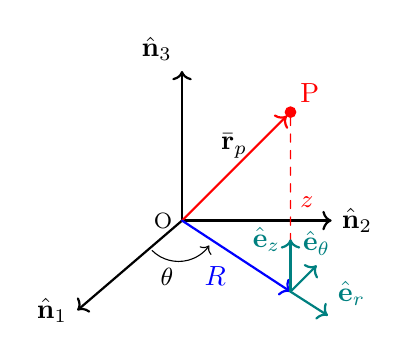
\begin{tikzpicture}[scale=0.95, line cap=round, line join=round]
            % origin
            \coordinate (O) at (0,0);
            \node at (O) [left] {\footnotesize$\text{O}$};

            % inertial (N) axes
            \draw[->, thick] (O) -- (-1.4,-1.2) node[left]  {$\hat{\mathbf n}_1$};
            \draw[->, thick] (O) -- ( 2.0, 0.0) node[right] {$\hat{\mathbf n}_2$};
            \draw[->, thick] (O) -- ( 0.0, 2.0) node[above left] {$\hat{\mathbf n}_3$};

            % % body (B) axes
            % \draw[->, thick, blue] (O) -- ( -0.4,-1.4) node[below right] {$\hat{\mathbf b}_1$};
            % \draw[->, thick, blue] (O) -- ( 1.8, 0.8) node[above right] {$\hat{\mathbf b}_2$};
            % \draw[->>, thick, blue] (O) -- ( 0.0, 2.0) node[above right] {$\hat{\mathbf b}_3$};

            % % angle between b2 and n2
            % \draw[->] (0.9,0.0) arc[start angle=0, end angle=23, radius=0.9];
            % \node at (1.1,0.25) {\scriptsize$\theta$};

            % add vector r_p
            \draw[->, thick, red] (O) -- (1.4,1.4);
            \node at (1.0,1.0) [left] {$\bar{\mathbf r}_p$};
            % add point P at the end
            \filldraw[red] (1.45,1.45) circle (2pt) node[above right] {P};

            % projection of P on N1N2 plane and cylindrical frame E
            \coordinate (R) at (1.45,-0.95);
            \draw[->, thick, blue] (O) -- (R) node[midway, below left] {$R$};
            % \filldraw[red] (R) circle (2pt) node[below left] {$R$};
            \draw[red, dashed] (R) -- (1.45,1.45) node[midway, right] {\small$z$};

            % angle theta
            \draw[->] (-0.4,-0.4) arc[start angle=-135, end angle=-35, radius=0.5];
            \node at (-0.2,-0.75) {\small$\theta$};

            % frame E at the end of R (cylindrical)
            \draw[->, thick, teal] (R) -- ($(R)+(0.5,-0.32)$) node[above right] {$\hat{\mathbf e}_r$};
            \draw[->, thick, teal] (R) -- ($(R)+(0.35,0.35)$) node[above] {$\hat{\mathbf e}_\theta$};
            \draw[->, thick, teal] (R) -- ($(R)+(0,0.7)$) node[left] {$\hat{\mathbf e}_z$};
        \end{tikzpicture}
    \end{flushright}
\end{frame}

\begin{frame}[t]{}

\end{frame}

\begin{frame}{Writing a DCM for a Simple Rotation}
    Steps for a simple rotation DCM:
    \begin{enumerate}
    \item Identify the axis of rotation (here: $\hat{\mathbf n}_3 \equiv \hat{\mathbf e}_z$).
    \item Visualize in 2D by looking through the axis of rotation.
    \end{enumerate}

    \begin{flushleft}
        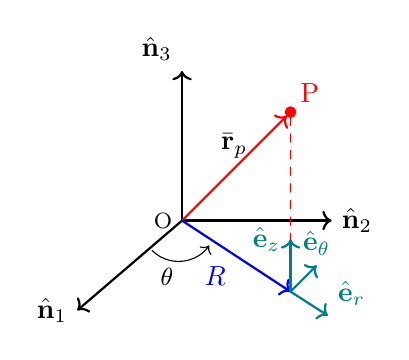
\begin{tikzpicture}[scale=0.95, line cap=round, line join=round]
            % origin
            \coordinate (O) at (0,0);
            \node at (O) [left] {\footnotesize$\text{O}$};

            % inertial (N) axes
            \draw[->, thick] (O) -- (-1.4,-1.2) node[left]  {$\hat{\mathbf n}_1$};
            \draw[->, thick] (O) -- ( 2.0, 0.0) node[right] {$\hat{\mathbf n}_2$};
            \draw[->, thick] (O) -- ( 0.0, 2.0) node[above left] {$\hat{\mathbf n}_3$};

            % % body (B) axes
            % \draw[->, thick, blue] (O) -- ( -0.4,-1.4) node[below right] {$\hat{\mathbf b}_1$};
            % \draw[->, thick, blue] (O) -- ( 1.8, 0.8) node[above right] {$\hat{\mathbf b}_2$};
            % \draw[->>, thick, blue] (O) -- ( 0.0, 2.0) node[above right] {$\hat{\mathbf b}_3$};

            % % angle between b2 and n2
            % \draw[->] (0.9,0.0) arc[start angle=0, end angle=23, radius=0.9];
            % \node at (1.1,0.25) {\scriptsize$\theta$};

            % add vector r_p
            \draw[->, thick, red] (O) -- (1.4,1.4);
            \node at (1.0,1.0) [left] {$\bar{\mathbf r}_p$};
            % add point P at the end
            \filldraw[red] (1.45,1.45) circle (2pt) node[above right] {P};

            % projection of P on N1N2 plane and cylindrical frame E
            \coordinate (R) at (1.45,-0.95);
            \draw[->, thick, blue] (O) -- (R) node[midway, below left] {$R$};
            % \filldraw[red] (R) circle (2pt) node[below left] {$R$};
            \draw[red, dashed] (R) -- (1.45,1.45);

            % angle theta
            \draw[->] (-0.4,-0.4) arc[start angle=-135, end angle=-35, radius=0.5];
            \node at (-0.2,-0.75) {\small$\theta$};

            % frame E at the end of R (cylindrical)
            \draw[->, thick, teal] (R) -- ($(R)+(0.5,-0.32)$) node[above right] {$\hat{\mathbf e}_r$};
            \draw[->, thick, teal] (R) -- ($(R)+(0.35,0.35)$) node[above] {$\hat{\mathbf e}_\theta$};
            \draw[->, thick, teal] (R) -- ($(R)+(0,0.7)$) node[left] {$\hat{\mathbf e}_z$};
        \end{tikzpicture}
    \end{flushleft}
\end{frame}

\begin{frame}[t]{What about Acceleration?}

\end{frame}

\begin{frame}[t]{Example: Tug-of-War on a Rotating Platform}
    In a game of Tug-of-War, participants are constrained to move only along a narrow platform. Moreover, the platform is rotating at angular velocity $\dot\theta\,\hat{\mathbf n}_3$. They move back and forth so that the distance from the center of the platform to a point $P$ (point mass) is given by
    \[
    r(t)=\frac{a}{2}\Big(1+\sin(\omega t)\Big)
    \]
    Find the \emph{inertial} acceleration of $P$.
    \vspace{0.25cm}
    \begin{center}
    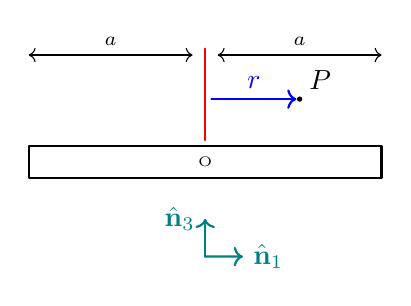
\begin{tikzpicture}[scale=0.8, line cap=round, line join=round]
        % platform (top view)
        \coordinate (O) at (0,0);
        \node at (O) {\tiny$\text{O}$};
        \coordinate (OO) at (0, -1.5);

        % inertial axes
        \draw[->, thick, teal] (OO) -- (0.6,-1.5) node[right] {$\hat{\mathbf n}_1$};
        \draw[->, thick, teal] (OO) -- (0,-0.9) node[left] {$\hat{\mathbf n}_3$};

        % platform rectangle (rotating about n3, sketched as a bar)
        \draw[thick] (-2.8,0.25) -- (2.8,0.25) -- (2.8,-0.25) -- (-2.8,-0.25) -- cycle;

        % point P on platform
        \coordinate (P) at (1.5,1.0);
        \fill (P) circle (1.2pt) node[above right] {$P$};

        % r arrow
        \draw[->, thick, blue] (0.1,1.0) -- (1.45,1.0) node[midway, above] {$r$};

        % "electric fence" sketch
        \draw[thick, red] (0.0,1.8) -- (0.0,0.35);

        % half-length markers a (illustrative)
        \draw[<->] (-2.8,1.7) -- (-0.2,1.7) node[midway, above] {\scriptsize $a$};
        \draw[<->] (0.2,1.7) -- (2.8,1.7) node[midway, above] {\scriptsize $a$};
    \end{tikzpicture}
    \end{center}
\end{frame}

\begin{frame}{Step 1: Define Frames}

\end{frame}

\begin{frame}[t]{Step 2: Write the DCM}
    \begin{enumerate}
        \item Identify the axis of rotation (here: $\hat{\mathbf n}_3$).
        \item Visualize in 2D by looking through the axis of rotation.
    \end{enumerate}

\end{frame}

\begin{frame}{Step 3: Position, Velocity, and Acceleration of $P$}

\end{frame}

\begin{frame}{Step 3: ...Continued}

\end{frame}

\begin{frame}{Summary}
    \begin{itemize}
        \item Reference frames are essential to describe motion
        \item Direction Cosine Matrices (DCMs) allow us to convert vectors between frames
        \begin{enumerate}
            \item Identify the axis of rotation
            \item Visualize in 2D by looking through the axis of rotation
        \end{enumerate}
        \item Velocity and acceleration in rotating frames have additional terms
    \end{itemize}
\end{frame}

\end{document}
